% !TeX root = surprises.tex

\chapter{Trisection of an Angle}\label{c.trisect}

%%%%%%%%%%%%%%%%%%%%%%%%%%%%%%%%%%%%%%%%%%%%%%%%%%%%%%%%%%%%%%%

\abstract*{It is impossible to trisect an angle using only a straightedge and compass. This was proved in by Pierre Wantzel in 1837. Nevertheless, innumerable amateurs continue to attempt to trisect an angle. This chapter presents two incorrect constructions and through trigonometry shows that the constructions are approximations.
The Greeks discovered that if other instruments are allowed, angles can be trisected. We bring Archimedes's construct using a simple instrument called a neusis and a more complex construction by Hippias using the quadratrix.
The rest of the chapter contains a somewhat informal proof of the impossibility of trisecting an angle by characterizing constructible numbers and then relating them constructible numbers to roots of polynomials which proves the impossibility.}

%%%%%%%%%%%%%%%%%%%%%%%%%%%%%%%%%%%%%%%%%%%%%%%%%%%%%%%%%%%%%%%

It is impossible to trisect an arbitrary angle (divide the angle into three equal parts) using only a straightedge and compass. Trisection requires the construction of cube roots, but a straightedge and compass can only construct lengths that are expressions built from integers, the four arithmetic operators and square roots. This was proved by Pierre Wantzel\index{Wantzel, Pierre} in 1837. Nevertheless, innumerable amateurs continue to attempt to trisect an angle. Their constructions are approximations though they are convinced that the constructions are correct. Section~\ref{s.trisect-approx} presents two such constructions, develops formulas for the angles and shows the errors in the approximations.

Greek mathematicians discovered that if other instruments are allowed, angles can be trisected. Section~\ref{s.neusis} explains a construction by Archimedes\index{Archimedes} using a simple instrument called a \emph{neusis} and Sect~\ref{s.neusis-doubling} shows how to double a cube using the neusis. Section~\ref{s.q} presents a construction for trisection by Hippias\index{Hippias} using an instrument called a \emph{quadratrix}. The rest of the chapter contains a proof of the impossibility of trisecting an angle. Section~\ref{s.trisect-constructible} characterizes constructible numbers, Sect.~\ref{s.trisect-poly} relates constructible numbers to roots of polynomials and Sect.~\ref{s.trisect-impossible} uses this theory to show that trisecting an angle and doubling a cube are impossible.

%%%%%%%%%%%%%%%%%%%%%%%%%%%%%%%%%%%%%%%%%%%%%%%%%%%%%%%%

\section{Approximate Trisections}\label{s.trisect-approx}

\subsection{First Approximate Trisection}\index{Trisection of an angle!approximation}\label{sub.trisect-approx1}

\noindent\textbf{Construction:}
Let $\theta=\angle AOB$ be an arbitrary angle and without loss of generality assume that $A,B$ are on a unit circle whose center is $O$. Bisect $\angle AOB$ and let $C$ be the intersection of the bisector with the unit circle. Let $D$ be the midpoint of $\overline{OA}$ and let $T$ be the midpoint of the $\overline{DC}$. Denote the angle $\angle DOT$ by $\phi$ (Fig.~\ref{f.trisect-first-approx-1}).

\newpage

\begin{figure}[ht]
\begin{center}
\begin{tikzpicture}[scale=.6]
\coordinate (O) at (0,0)
  node[left] {$O$}
  node[above right,xshift=14pt,yshift=16pt] {\sm{\theta/2}}
  node[right,xshift=18pt,yshift=4pt] {\sm{\theta/2}};
\coordinate (A) at (9cm,0);
\node[right] at (A) {$A$};
\coordinate (B) at (60:9);
\node[above] at (B) {$B$};
\draw (A) arc(0:60:9);
\draw (B) -- (O) -- (A);
\coordinate (C) at (30:9);
\node[right] at (C) {$C$};
\draw (O) -- node[above] {$1$} (C);
\coordinate (D) at (4.5,0);
\node[below] at (D) {$D$};
\coordinate (T) at ($(D)!.5!(C)$);
\draw (D) -- node[left] {$a$} (T) -- node[left] {$a$} (C);
\node[right] at (T) {$T$};
\draw (O) -- (T);
\draw (	1,0) arc (0:30:1);
\draw (30:.8) arc (30:60:.8);
\draw (2,0) arc (0:20:2);
\node[above right] at (2.1,0.1) {\sm{\phi}}; 

\draw[<->] (0,-1) -- node[fill=white] {$1/2$} +(4.5,0);
\draw[<->] (4.5,-1) -- node[fill=white] {$1/2$} +(4.5,0);
\end{tikzpicture}
\end{center}
\caption{First approximate trisection (1)}\label{f.trisect-first-approx-1}
\end{figure}


\begin{theorem}
\[\tan\phi =\frac{2\sin(\theta/2)}{1+2\cos(\theta/2)}\,.\]
\end{theorem}

\begin{proof} Figure~\ref{f.trisect-first-approx-2} is extracted from Fig.~\ref{f.trisect-first-approx-1} and contains additional annotations.

Let $\overline{CF}$ be the perpendicular to $\overline{OA}$ that intersects $\overline{OA}$ at $F$. Since $\overline{OC}=1$, $\overline{CF}=\sin (\theta/2)$ and $\overline{OF}=\cos(\theta/2)$. Let $\overline{TE}$ be the perpendicular to $\overline{OA}$ that intersects $\overline{OA}$ at $E$.

$T$ is the midpoint of $\overline{DC}$ so $\overline{DT}=\overline{TC}=a$. But $\overline{FT}$ is the median to the hypotenuse of a right triangle, so $\overline{FT}=a$ and therefore $\triangle DTF$ is isoceles. It follows that $\overline{TE}$ is the both the median and the altitude of $\overline{DF}$. From the diagram it is easy to see that:
\begin{figure}[ht]
\begin{center}
\begin{tikzpicture}[scale=.9]
\coordinate (O) at (0,0)
  node[left] {$O$}
  node[right,xshift=24pt,yshift=5pt] {\sm{\theta/2}};
\coordinate (A) at (9cm,0);
\node[right] at (A) {$A$};
\draw (O) -- (A);
\coordinate (C) at (30:9);
\node[right] at (C) {$C$};
\draw (O) -- node[above] {$1$} (C);
\coordinate (D) at (4.5,0);
\node[below] at (D) {$D$};
\coordinate (T) at ($(D)!.5!(C)$);
\draw (D) -- node[left] {$a$} (T) -- node[left] {$a$} (C);
\node[right] at (T) {$T$};
\draw (O) -- (T);
\draw (	1,0) arc (0:30:1);
\draw (2,0) arc (0:20:2);
\node[above right] at (1.9,0.1) {\sm{\phi}}; 

\coordinate (E) at (T |- A);
\draw[thick,dashed] (T) -- node[right] {$h$}
  (E) node[below] {$E$};
\draw[rotate=90] (E) rectangle +(7pt,7pt);

\coordinate (F) at (C |- A);
\draw[thick,dashed] (C) --
  node[right] {$\sin (\theta/2)$} (F) node[below] {$F$};
\draw[rotate=90] (F) rectangle +(7pt,7pt);

\draw[thick,dashed] (T) -- node[right] {$a$} (F);

\draw[<->] ($(O)+(0,-1)$) --
  node[fill=white] {$1/2$} +(4.5,0);
\draw[<->] ($(O)+(0,-1.8)$) --
  node[fill=white] {$\cos (\theta/2)$} ($(F)+(0,-1.8)$);
\draw[<->] ($(D)+(0,-2.6)$) --
  node[fill=white] {$\left(\cos (\theta/2)\!-\! (1/2)\right)$} 
  ($(F)+(0,-2.6)$);
\draw[<->] ($(O)+(0,-3.4)$) --
  node[fill=white] {$(1/2)+(1/2)\left(\cos (\theta/2)\! -\! (1/2)\right)$} 
  ($(E)+(0,-3.4)$);
\end{tikzpicture}
\end{center}
\caption{First approximate trisection (2)}\label{f.trisect-first-approx-2}
\end{figure}
\[
\overline{OE}=\frac{1}{2} + \frac{1}{2}\left(\cos \frac{\theta}{2}-\frac{1}{2}\right)\,.
\]
Compute the length $2a=\overline{CD}$ using Pythagoras's Theorem in $\triangle DCF$:
\begin{eqnarray*}
(2a)^2 &=&  \left(\cos \frac{\theta}{2}-\frac{1}{2}\right)^2+\sin^2\frac{\theta}{2}\,.
\end{eqnarray*}

\newpage

The length $h=\overline{TE}$ can be computed from Pythagoras's Theorem in $\triangle DTE$:
\begin{eqnarray*}
a^2 &=& h^2 + \left[\frac{1}{2}\left(\cos \frac{\theta}{2}-\frac{1}{2}\right)\right]^2\\
h^2&=&\frac{1}{4}\left(\cos \frac{\theta}{2}-\frac{1}{2}\right)^2+\frac{1}{4}\sin^2\frac{\theta}{2}-\left[\frac{1}{2}\left(\cos \frac{\theta}{2}-\frac{1}{2}\right)\right]^2=
\frac{1}{4}\sin^2\frac{\theta}{2}\\
h&=&\frac{1}{2}\sin\frac{\theta}{2}\\
\tan\phi &=&\frac{h}{\overline{OE}}=\displaystyle\frac{\displaystyle\frac{1}{2}\sin\frac{\theta}{2}}{\displaystyle\frac{1}{2}+\frac{1}{2}\left(\cos \frac{\theta}{2}\! -\! \frac{1}{2}\right)}
=\frac{\displaystyle2\sin\frac{\theta}{2}}{\displaystyle 1+2\cos\frac{\theta}{2}}\,.
\end{eqnarray*}                  
\end{proof}

This is an approximation to a trisection $\phi=\theta/3$. For $\theta=60^\circ$:
\[
\tan^{-1}\left(\frac{2\sin 30^\circ}{1+2\cos 30^\circ}\right)=
\tan^{-1}0.366\approx 20.1^\circ\approx 20^\circ\,.
\]

Table~\ref{t.trisect-first} shows the errors for a range of acute angles. The error is relatively small for small angles, rising to $1\%$ at $85^\circ$.

\begin{table}[t]
\caption{Errors in the first approximate trisection}\label{t.trisect-first}
\[
%
\begin{array}{r@{\hspace{5mm}}r@{\hspace{5mm}}r@{\hspace{5mm}}r@{\hspace{5mm}}r}
\hline
\noalign{\smallskip}
\theta ({}^\circ) & \theta/3 ({}^\circ)& \tan^{-1} \phi ({}^\circ) & \mathrm{Error} ({}^\circ) & \mathrm{Error (\%)}\\\svhline
\noalign{\smallskip}
  5 &    1.667 &    1.667  &     0.000 &    0.004 \\
 10 &    3.333 &    3.334  &     0.000 &    0.014 \\
 15 &    5.000 &    5.002  &     0.002 &    0.032 \\
 20 &    6.667 &    6.670  &     0.004 &    0.057 \\
 25 &    8.333 &    8.341  &     0.007 &    0.088 \\
 30 &   10.000 &   10.013  &     0.013 &    0.128 \\
 35 &   11.667 &   11.687  &     0.020 &    0.174 \\
 40 &   13.333 &   13.364  &     0.030 &    0.228 \\
 45 &   15.000 &   15.043  &     0.043 &    0.289 \\
 50 &   16.667 &   16.726  &     0.060 &    0.358 \\
 55 &   18.333 &   18.413  &     0.080 &    0.435 \\
 60 &   20.000 &   20.104  &     0.104 &    0.520 \\
 65 &   21.667 &   21.799  &     0.133 &    0.612 \\
 70 &   23.333 &   23.500  &     0.166 &    0.713 \\
 75 &   25.000 &   25.206  &     0.206 &    0.823 \\
 80 &   26.667 &   26.918  &     0.251 &    0.941 \\
 85 &   28.333 &   28.636  &     0.303 &    1.068 \\
 \noalign{\smallskip}
 \hline
 \end{array}
\]
\end{table}

\subsection{Second Approximate Trisection}\index{Trisection of an angle!approximation}

\noindent\textbf{Construction:}
Let $\theta=\angle AOB$ be an arbitrary angle and without loss of generality assume that $A,B$ are on a unit circle whose center is $O$. Construct a circle of radius $1/3$ with center $O$ and let $D$ be its intersection with $\overline{OA}$. Bisect $\angle AOB$ and let $C$ be the intersection of the bisector with the circle of radius $1/3$. Construct the chord $\overline{CD}$ and the chords $\overline{AE}=\overline{ET}=\overline{CD}$. Since equal chords subtend equal central angles $\angle TOE=\angle EOA=\phi$ (Fig.~\ref{f.trisect-second-approx}).

\begin{figure}[ht]
\begin{center}
\begin{tikzpicture}[scale=.75]
\coordinate (O) at (0,0)
  node[left] {$O$}
  node[above right,xshift=10pt,yshift=12pt] {\sm{\theta/2}};

\coordinate (A) at (9cm,0);
\node[right] at (A) {$A$};
\coordinate (B) at (60:9);
\node[above] at (B) {$B$};
\draw (A) arc(0:60:9);
\draw (B) -- (O) -- (A);
\coordinate (D) at (3,0);
\node[below] at (D) {$D$};
\draw[name path=third] (D) arc(0:60:3);
\coordinate (C) at (30:3);
\node[right] at (C) {$C$};
\draw (O) -- node[above,near end] {\sm{1/3}} (C);
\draw[thick] (D) -- (C);
\coordinate (E) at (10:9);
\node[right] at (E) {$E$};
\draw[thick] (A) -- node[right] {\sm{1/3}} (E);
\coordinate (T) at (20:9);
\node[right] at (T) {$T$};
\draw[thick] (E) -- node[right] {\sm{1/3}} (T);
\draw (O) -- node[above,near end] {$1$} (T);

\draw (	1,0) arc (0:30:1);
\draw (30:.8) arc (30:60:.8);
\draw (4,0) arc (0:20:4);
\node at (4.2,0.35) {$\phi$}; 
\node at (4.1,1.1) {$\phi$}; 

\draw[dashed] (O) --
  node[fill=white,inner sep=0pt,very near start,
       xshift=7pt,yshift=1pt] {\sm{\theta/2}} 
  node[fill=white,near end] {$1$} (E);

\draw[<->] (3,-.8) -- node[fill=white] {$2/3$} +(6,0);
\draw[<->] (0,-.8) -- node[fill=white] {$1/3$} +(3,0);
\end{tikzpicture}
\end{center}
\caption{Second approximate trisection}
\label{f.trisect-second-approx}
\end{figure}

\begin{theorem}
\[
\cos\phi=1 - \frac{1}{9}(1-\cos(\theta/2))=1 - \frac{2}{9}\sin^2(\theta/4)\,.
\]
\end{theorem}

\begin{proof} By the Law of Cosines in $\triangle DOC$:
\[
\overline{CD}= \left(\frac{1}{3}\right)^2+\left(\frac{1}{3}\right)^2-2\left(\frac{1}{3}\right)\left(\frac{1}{3}\right)\cos (\theta/2)=\frac{2}{9}(1-\cos(\theta/2))\,.
\]

By the Law of Cosines in $\triangle EOA$:
\[
\overline{AE} = 1^2+1^2-2\cdot 1\cdot 1\cdot \cos \phi=2(1-\cos \phi)\,.
\]

\newpage

Equating the two expressions for $\overline{CD}=\overline{AE}$ and simplifying we get:
\[
\cos \phi = 1 - \frac{1}{9}(1-\cos(\theta/2))\,.
\]
Since $\cos 2\alpha= \cos^2 \alpha-\sin^2\alpha=1-2\sin^2\alpha$, and therefore $1-\cos 2\alpha=2\sin^2\alpha$, we have the alternate formula:
\[
\cos \phi = 1 - \frac{2}{9}\sin^2(\theta/4)\,.
\]
\end{proof}

This is an approximation to a trisection $2\phi=\theta/3$. For $\theta=60^\circ$:
\[
2\cos^{-1}\left(1 - \frac{1}{9}(1-\cos 30^\circ)\right)\approx 19.8^\circ\approx 20^\circ\,.
\]

Table~\ref{t.trisect-second-approx} shows the errors for a range of acute angles. This construction is much less accurate than the one in Sect.~\ref{sub.trisect-approx1}.

\begin{table}[t]
\caption{Errors in the second approximate trisection}\label{t.trisect-second-approx}
\[
%
\begin{array}{r@{\hspace{5mm}}r@{\hspace{5mm}}r@{\hspace{5mm}}r@{\hspace{5mm}}r}
\hline
\noalign{\smallskip}
\theta ({}^\circ) & \theta/3 ({}^\circ)& \cos^{-1} 2\phi ({}^\circ) & \mathrm{Error} ({}^\circ) & \mathrm{Error (\%)}\\
\noalign{\smallskip}\svhline\noalign{\smallskip}
  5 &    1.667 &    1.667  &     0.000 &    0.007 \\
 10 &    3.333 &    3.332  &     0.001 &    0.028 \\
 15 &    5.000 &    4.997  &     0.003 &    0.063 \\
 20 &    6.667 &    6.659  &     0.008 &    0.113 \\
 25 &    8.333 &    8.319  &     0.015 &    0.176 \\
 30 &   10.000 &    9.975  &     0.025 &    0.254 \\
 35 &   11.667 &   11.626  &     0.040 &    0.346 \\
 40 &   13.333 &   13.273  &     0.060 &    0.451 \\
 45 &   15.000 &   14.914  &     0.086 &    0.571 \\
 50 &   16.667 &   16.549  &     0.118 &    0.705 \\
 55 &   18.333 &   18.177  &     0.156 &    0.853 \\
 60 &   20.000 &   19.797  &     0.203 &    1.015 \\
 65 &   21.667 &   21.408  &     0.258 &    1.192 \\
 70 &   23.333 &   23.011  &     0.322 &    1.382 \\
 75 &   25.000 &   24.603  &     0.397 &    1.586 \\
 80 &   26.667 &   26.185  &     0.481 &    1.805 \\
 85 &   28.333 &   27.756  &     0.577 &    2.038 \\
 \noalign{\smallskip}
 \hline
 \end{array}
\]
\end{table}


%%%%%%%%%%%%%%%%%%%%%%%%%%%%%%%%%%%%%%%%%%%%%%%%%%%%%%%%%%%%

\newpage

\section{Trisection Using a Neusis}\label{s.neusis}\index{Trisection of an angle!neusis@with a neusis}
\index{Neusis!trisection of an angle}

The term \emph{straightedge} is used instead of \emph{ruler} because a straightedge has no marks on it. It can only be used to construct a straight line between two given points. Archimedes\index{Archimedes} showed that a \emph{neusis}, a straightedge with two marks that are a fixed distance apart, can be used to trisect an angle (Fig.~\ref{f.neusis}). We define the distance between the marks to be $1$.

\begin{figure}[b]
\begin{center}
\begin{tikzpicture}[scale=3.5]
\draw (-1,1.05) rectangle +(3.2,.1);
\draw[thick] (1.89,1.05) -- +(0,.1);
\draw[thick] (.73,1.05) -- +(0,.1);
\draw[<->] (.73,1.25) -- node[fill=white] {$1$} (1.89,1.25);
\end{tikzpicture}
\end{center}
\caption{A neusis}\label{f.neusis}
\end{figure}

\begin{figure}[t]
\begin{center}
\begin{tikzpicture}[scale=2.1]
\coordinate (origin) at (0,0) node[below] {$B$} ;
\draw[name path=circle] (origin) circle [radius=1];
\draw (origin) node[above left,xshift=-4pt] {$\alpha$} -- node[fill=white] {$1$} (120:1) coordinate (a) node[below,xshift=-2pt] {$A$} ;
\draw (-1,0) -- (2.5,0);
\path[name path=ad] (a) -- (0,0 -| 2,0) coordinate (d) node[below] {$D$} ;
\path[name intersections={of=circle and ad,by={c,a1}}];
\coordinate (e) at (-1,0);
\vertex{origin};
\node [below,xshift=-4pt] at (c) {$C$};
\node [left] at (e) {$E$};
\node at (1.5,2.5pt) {$\beta$};
\begin{scope}[rotate=-19,yshift=-11.25pt]
\draw (-1,1.05) rectangle +(3.2,.1);
\draw[thick] (1.89,1.05) -- +(0,.1);
\draw[thick] (.76,1.05) -- +(0,.1);
\draw[<->] (.73,1.3) -- node[fill=white] {$1$} (1.89,1.3);
\end{scope}
\end{tikzpicture}
\end{center}
\caption{The neusis construction for trisecting an angle (1)}\label{f.trisect-neusis-1}
\end{figure}
\noindent\textbf{Construction:}
Let $\alpha=\angle ABE$ be an arbitrary angle in a unit circle with center $B$, where the radius of the circle equals the distance between the marks on the neusis. Extend the radius $\overline{EB}$ beyond the circle. Place an edge of the neusis on $A$ and move it until it intersects the extension of $\overline{EB}$ at $D$ and the circle at $C$, using the marks so that the length of the line segment $\overline{CD}$ is $1$.\footnote{This operation is called \emph{verging}.} Construct the line $\overline{AD}$. Denote $\angle CDB=\beta$ (Fig.~\ref{f.trisect-neusis-1}).

\begin{theorem} $\beta=\alpha/3$.
\end{theorem}
\begin{proof}
Construct $\overline{BC}$ and denote the angles and line segments as shown in Fig.~\ref{f.trisect-neusis-2}.
$\triangle ABC$ and $\triangle BCD$ are isoceles triangles: $\overline{AB} = \overline{BC}$ are radii of the same circle and $\overline{BC} = \overline{CD}$ by construction using the neusis. Since the sum of the angles of a triangle is equal to $180^\circ$ and the sum of supplementary angles is also equal to $180^\circ$, we have:
\begin{eqnarray*}
\epsilon &=& 180^\circ - 2\beta\\
\gamma &=& 180^\circ - \epsilon = 2\beta\\
\delta &=& 180^\circ - 2\gamma = 180^\circ - 4\beta\\
\alpha &=& 180^\circ - \delta - \beta=3\beta\,.
\end{eqnarray*}
\end{proof}

\begin{figure}[tbh]
\begin{center}
\begin{tikzpicture}[scale=2.1]
\coordinate (origin) at (0,0) node[below] {$B$} ;
\draw[name path=circle] (origin) circle [radius=1];
\draw (origin)
  node[above left,xshift=-4pt] {$\alpha$}
  node[above,xshift=4pt,yshift=2pt] {$\delta$}
  node[above right,xshift=30pt,yshift=-2pt] {$\beta$} --
  node[fill=white] {$1$} (120:1)
  coordinate (a) node[above left] {$A$};
\draw (-1,0) -- (2.2,0);
\draw[name path=ad] (a)
  node[below right,xshift=8pt,yshift=-6pt] {$\gamma$} -- 
  (0,0 -| 2,0) coordinate (d)
  node[left,xshift=-24pt,yshift=5pt] {$\beta$}
  node[above right] {$D$};
\path[name intersections={of=circle and ad,by={c,a1}}];
\draw (origin) -- node[fill=white] {$1$}(c) node[above right] {$C$} node[left,xshift=-12pt] {$\gamma$} node[below,xshift=-2pt,yshift=0pt] {$\epsilon$};
\coordinate (e) at (-1,0);
\vertex{origin};
\node [left] at (e) {$E$};
\path (c) -- node[fill=white,near start] {$1$} (d);
\end{tikzpicture}
\end{center}
\caption{The neusis construction for trisecting an angle (2)}\label{f.trisect-neusis-2}
\end{figure}

%%%%%%%%%%%%%%%%%%%%%%%%%%%%%%%%%%%%%%%%%%%%%%%%%%%%%%%%%%%%%

\newpage

\section{Doubling the Cube with a Neusis}\label{s.neusis-doubling}

Given a cube $C$ construct another cube with twice its volume. If the volume of $C$ is $V$ its sides are of length $\sqrt[3]{V}$. The sides of a cube with twice the volume are $\sqrt[3]{2 V}=\sqrt[3]{2}\cdot\sqrt[3]{V}$, so if we can construct $\sqrt[3]{2}$ we can double the cube.

\smallskip

\noindent\textbf{Construction:}
Construct the unit equilateral triangle $\triangle ABC$ and extend $\overline{CA}$ with another unit line segment to $D$. Construct rays extending $\overline{AB}$ and $\overline{DB}$. Place the neusis on point $C$ and move it until one mark on the neusis is placed on the ray $\overline{AB}$ at $P$ and the other mark is placed on the ray $\overline{DB}$ at $Q$. Denote $\overline{CQ}=x$ and $\overline{BP}=y$ (Fig.~\ref{f.double-neusis}).

\begin{figure}[b]
\begin{center}
\begin{tikzpicture}[scale=.7]
\clip (-.5,-.4) rectangle +(11,6.5);
\coordinate (D) at (0,0) node[left] {$D$};
\draw (D) -- ++(60:6) coordinate (C) node[above] {$C$};
\coordinate (A) at (60:3);
\node[left] at (A) {$A$};
\draw (A) -- ++(3,0) coordinate (B) -- (C);
\node[below right] at (B) {$B$};
\path[name path=DQ] (D) -- ($(D)!1.7!(B)$);
\path[name path=AP] (A) -- ($(A)!3!(B)$);
% 3*(1+\sqrt[3]{2}) = 6.78
\path[name path=CP] (C) circle (6.78cm);
\path[name intersections={of=CP and AP,by={P}}];
\draw[name path=CP] (C) -- (P);
\path[name intersections={of=CP and DQ,by={Q}}];
\node[above] at (Q) {$Q$};
\node[right] at (P) {$P$};
\draw (D) -- (Q);
\draw (B) -- (P);
\path (D) -- node[left] {$1$} (A) -- node[left] {$1$} (C) --
  node[right] {$1$} (B) -- node[below] {$1$} (A);
\path (C) -- node[above] {$x$} (Q) -- node[above] {$1$} (P) -- 
  node[below] {$y$} (B);
\end{tikzpicture}
\end{center}
\caption{Doubing the cube with a neusis}\label{f.double-neusis}
\end{figure}

\begin{theorem}\index{Doubling a cube!neusis@with a neusis}
\index{Neusis!doubling of a cube}
$x=\sqrt[3]{2}$.
\end{theorem}

\begin{proof}
Since $\triangle ABC$ is equilateral, $\cos \angle CAP=\cos 60^\circ=\frac{1}{2}$ and by the Law of Cosines\index{Law of cosines} in $\triangle APC$:
\begin{subeqnarray}
\overline{CP}&=&\overline{AC}^2+\overline{AP}^2-2\cdot \overline{AC}\cdot\overline{AP}\cos 60^\circ\\
(x+1)^2&=&1^2+(y+1)^2-2\cdot 1\cdot (y+1)\cdot \frac{1}{2}\\
x^2+2x&=&y^2+y\slabel{eq.eq-cube-double}\,.
\end{subeqnarray}

By Menelaus's theorem (Thm.~\ref{thm.menelaus}):
\[
\displaystyle\frac{\overline{AB}}{\overline{BP}}\cdot
\displaystyle\frac{\overline{PQ}}{\overline{QC}}\cdot
\displaystyle\frac{\overline{CD}}{\overline{DA}}=1\,.
\]

\newpage

Therefore:
\begin{subeqnarray}
\displaystyle\frac{1}{y}\cdot
\displaystyle\frac{1}{x}\cdot
\displaystyle\frac{2}{1}&=&1\\
xy&=&2\,.\slabel{eq.menelaus-xy2}
\end{subeqnarray}

Substituting Eq.~\ref{eq.menelaus-xy2} into Eq.~\ref{eq.eq-cube-double} gives:
\begin{eqnarray*}
x^2+2x&=&\frac{4}{x^2}+\frac{2}{x}\\
x^4+2x^3&=&4+2x\\
x^3(x+2)&=&2(x+2)\\
%x^3&=&2\\
x&=&\sqrt[3]{2}\,.
\end{eqnarray*}
\end{proof}


%%%%%%%%%%%%%%%%%%%%%%%%%%%%%%%%%%%%%%%%%%%%%%%%%%%%%%%%%%%%%
\section{Trisection Using a Quadratrix}\label{s.q}

\index{Trisection of an angle!quadratrix@with a quadratrix}

Let $\overline{ABCD}$ be a square. Let $l_1$ be a line segment placed initially at $\overline{DC}$ and let $l_2$ be a line segment placed initially at $\overline{AD}$. Move $l_1$ move at a constant linear velocity until it reaches $\overline{AB}$ and rotate $l_2$ at a constant angular velocity clockwise on $A$ until it also reaches $\overline{AB}$. Assume that they reach $\overline{AB}$ together. For example, if $l_2$ rotates at $1^\circ$/second and the side of the square is $9$ centimeters, $l_1$ must move at $0.1$ cm/second. The trace of their point of intersection $P$ is called a \emph{quadratrix curve}\index{Quadratrix} or simply a \emph{quadratrix} (Fig.~\ref{f.trisect-quad-curve}). Its definition is attributed to the mathematician Hippias\index{Hippias}.

\begin{figure}[b]
\subfigures
\leftfigure[c]{
\begin{tikzpicture}[scale=.6,domain=.03:1.555,samples=100]
\draw (.1,.2)
  node[below left,xshift=-8pt] {$A$} -- 
  (7.8,.2) 
  node[below right] {$B$} -- 
  (8,7.8) 
  node[above right] {$C$} -- 
  (.1,7.8) node[above left,xshift=-8pt] {$D$} -- 
  cycle;
\draw[thick,dashed,name path=arm] (.1,.2) -- node[right,very near end] {$l_2$} (59.6:7.9);
\draw[thick,dashed,name path=horiz] (.1,5) -- node[above,near end] {$l_1$} +(7.8,0);
\path[name intersections={of=arm and horiz,by={A}}];
\node[above left,xshift=-2pt] at (A) {$P$};
\vertex{A};
\draw[thick] plot (4.6*.637*\x,{12.2*.637*\x*cot(\x r)});
\end{tikzpicture}
}
\hfill
\rightfigure[c]{
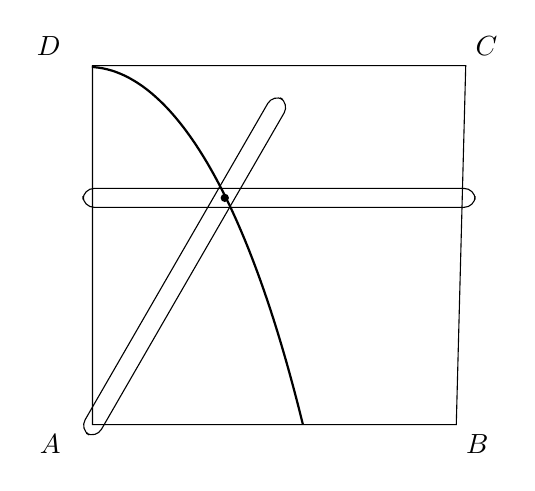
\begin{tikzpicture}[scale=.6,domain=.03:1.555,samples=100]
\draw (.1,.2) node[below left,xshift=-8pt] {$A$} -- (7.8,.2) node[below right] {$B$} -- (8,7.8) node[above right] {$C$} -- (.1,7.8) node[above left,xshift=-8pt] {$D$} -- cycle;
\draw[rounded corners,rotate=60] (0,-.2) rectangle (8.2,.2);
\draw[rounded corners] (-.1,4.8) rectangle (8.2,5.2);
\fill (2.9,5) circle [radius=2.5pt];
\draw[thick] plot (4.6*.637*\x,{12.2*.637*\x*cot(\x r)});
\end{tikzpicture}
}
\leftcaption{A quadratrix curve}\label{f.trisect-quad-curve}
\rightcaption{A quadratrix compass}\label{f.trisect-quad-compass}
\end{figure}

A quadratrix can be constructed using a \emph{quadratrix compass}\index{Quadratrix!compass} as shown in Fig.~\ref{f.trisect-quad-compass}. It consists of two (unmarked) straightedges that move as described above. A joint constrains them to move together and traces out the curve.


\begin{figure}[b]
\begin{center}
\begin{tikzpicture}[scale=.8,domain=.03:1.562,samples=100]
\draw (.1,7.8) coordinate (start)
  node[above left] {$D$}
  node[below right,xshift=32pt] {$\theta$} -- 
  (.1,.2) node[below left] {$A$} -- 
  (8,.1)  node[below right] {$B$} -- 
  (8,7.8) node[above right] {$C$} -- 
  cycle;
\draw[name path=curve,thick] plot (4.6*.637*\x,{12.2*.637*\x*cot(\x r)});
% To ensure intersection at node D, path should extend to the upper left of D
\coordinate (twenty-a) at ($(start)+(-35:9)$);
\path[name path=twenty] ($(start)!-.1!(twenty-a)$) -- (twenty-a);
\path[name path=sixty] (start) -- +(-50:11);
\path[name path=xaxis] (.1,.2) -- (8,.1);
\path[name intersections={of=twenty and curve,by={x1,tri}}];
\draw (start) -- (tri);
\node[above right] at (tri) {$P_2$};
\path[name intersections={of=sixty and curve,by={x2,angle}}];
\node[above right] at (angle) {$P_1$};
\draw (start) -- (angle);
\path[name intersections={of=xaxis and curve,by=x}];
\path[name intersections={of=sixty and xaxis,by=sixty-x}];
\draw (start) -- (sixty-x);

\path (tri) -- (tri -| .1,.2) coordinate (t3);
\draw[dashed] (t3) -- +(7.9,0);
\node[left] at (t3) {$F$};
\path (angle) -- (angle -| .1,.2) coordinate (t);
\draw[dashed] (t) -- +(7.9,0);
\node[left] at (t) {$E$};
\draw[<->] (-1.2,7.8) -- node[fill=white] {$t/3$} (-1.2,7.8 |- t3);
\draw[<->] (-.6,7.8) -- node[fill=white] {$t$} (-.6,7.8 |- t);
\draw[<->] (-.6,7.8 |- t) -- node[fill=white] {$1-t$} (-.6,.2);
\draw (3.5,7.8) arc[start angle=0,delta angle=-49,radius=3.5];
\draw (1,7.8) arc[start angle=0,delta angle=-32,radius=1];
\node at (3.3,6) {$\alpha$}; 
\end{tikzpicture}
\end{center}
\caption{Trisection of an angle using a quadratrix}\label{f.trisect-quad-trisect}
\end{figure}

A quadratrix can be used to trisect an angle.

\noindent\textbf{Construction:}
Let $\angle CDP_1=\alpha$ be an arbitrary angle, where $P_1$ is the intersection of the line defining the angle $\alpha$ relative to $\overline{DC}$ and the quadratrix. Construct a line through $P_1$ parallel to $\overline{DC}$ and denote its intersection with $\overline{AD}$ by $E$. Denote the line segment $\overline{DE}$ by $t$ and trisect it (Sect.~\ref{s.trisect-constructible}) to obtain point $F$ that is $t/3$ from $\overline{DC}$. Let $P_2$ be the intersection of a line from $F$ parallel to $\overline{DC}$ and the quadratrix, and denote by $\theta$ the angle between $\overline{DC}$ and $\overline{DP_2}$ (Fig.~\ref{f.trisect-quad-trisect}).

\begin{theorem}
$\theta = \alpha/3$.
\end{theorem}
\begin{proof}
$E$ has $y$-coordinate $1-t$ so by construction $F$ has $y$-coordinate $1-(t/3)$. Since the constant linear velocity of the horizontal line is proportional to the constant angular velocity of the rotating line $\theta/\alpha = (t/3)/t$ and $\theta = \alpha/3$.
\end{proof}

\newpage

\section{Constructible Numbers}\label{s.trisect-constructible}
\index{Constructible number}

Let $l$ be a line segment defined to be of length $1$.

\begin{definition}
A number $a$ is \emph{constructible} if and only if a line segment of length $a$ can be constructed with a straightedge and compass starting from $l$.
\end{definition}

Given line segment $l=\overline{AB}$, construct a line containing $\overline{AB}$ and use the compass to find a point $C$ on the line that is a distance of $1$ from $B$. Then $\overline{AC}$ is of length $2$ so the number $2$ is constructible. A line segment $\overline{BD}$ of length $1$ can be constructed perpendicular to $\overline{AB}$ at $B$. The hypotenuse of the triangle $\triangle ABD$ is of length $\sqrt{2}$ so the number $\sqrt{2}$ is constructible.

\begin{theorem}\label{thm.trisect-constructible}
A number is \emph{constructible} if and only if it is the value of an expression built from the integers, the four arithmetic operations $\{+,-,\times,/\}$ and the operation of taking a square root $\surd$.
\end{theorem}

\begin{proof} First we show that the values of these expressions are constructible.
\index{Constructible number!arithmetic operation}

\medskip

\begin{figure}[b]
\begin{center}
\begin{tikzpicture}[scale=.8]
\coordinate (P) at (0,0);
\coordinate (Q) at (5,0);
\coordinate (T) at (3,0);
\coordinate (U) at (7,0);
\vertex{P};
\vertex{Q};
\draw (P) -- (Q);
\node[above] at (P) {$P$};
\node[above left] at (Q) {$Q$};
\node[above left] at (U) {$U$};
\node[above right] at (T) {$T$};
\draw (5,0) -- (8,0);
\draw (5,0) circle[radius=2cm];
\draw (5,0) -- node[left] {$b$} ++(60:2cm);
\coordinate (R) at (9,-1);
\coordinate (S) at ($(9,-1) + (20:2cm)$);
\vertex{R};
\vertex{S};
\draw (R) node[above] {$R$} --
  node[below right] {$b$} (S)
  node[above] {$S$};
\draw[<->] (0,-.5) -- node[fill=white] {$a$} (5,-.5);
\draw[<->] (0,-1) -- node[fill=white] {$a-b$} (3,-1);
\draw[<->] (0,-1.5) -- node[fill=white] {$a+b$} (7,-1.5);
\end{tikzpicture}
\end{center}
\caption{Construction of addition and subtraction}\label{f.trisect-add-subtract}
\end{figure}

\noindent\textbf{Addition and subtraction:}
Given line segments $\overline{PQ}=a$ and $\overline{RS}=b$, construct a circle centered at $Q$ with radius $b$ (Fig.~\ref{f.trisect-add-subtract}). Extend $\overline{PQ}$ until it intersects the circle at $U$. Then $\overline{PTQU}$ is a line segment, where $\overline{PT}=a-b$ and $\overline{PU}=a+b$.

\newpage

\noindent\textbf{Multiplication:}
By similar triangles in Fig.~\ref{f.trisect-multiplication},
$(1/b)=(a/\overline{OA})$, so $\overline{OA}=ab$.

\medskip

\noindent\textbf{Division:}
By similar triangles in Fig.~\ref{f.trisect-division},
$(1/b)=(\overline{OD}/a)$, so $\overline{OD}=(a/b)$.

\begin{figure}[t]
\subfigures
\leftfigure[c]{
\begin{tikzpicture}[scale=.8]
\draw[name path=horz] (0,0) coordinate (o) -- (7,0);
\node[left] at (o) {$O$};
\coordinate (a) at (6,0);
\node[below]  at (a) {$A$};
\draw (o) -- (30:5.5);
\coordinate (c) at (30:3);
\coordinate (b) at (30:5);
\node[above] at (c) {$C$};
\node[above] at (b) {$B$};
\draw (a) -- (b);
\path[name path=par] (c) -- +($(a)-(b)$);
\path[name intersections={of=par and horz,by=d}];
\node[below] at (d) {$D$};
\draw (c) -- (d);
\draw[<->] (-.4,.5) -- node[fill=white] {$b$} +(30:5.2);
\path (o) -- node[above] {$1$} (c);
\draw[<->] (0,-.8) -- node[fill=white] {$ab$} +(6,0);
\path (o) -- node[below] {$a$} (d);
\end{tikzpicture}
}
\hfill
\rightfigure[c]{
\begin{tikzpicture}[scale=.8]
\draw[name path=horz] (0,0) coordinate (o) -- (7,0);
\node[left] at (o) {$O$};
\coordinate (a) at (6,0);
\node[below]  at (a) {$A$};
\draw (o) -- (30:5.5);
\coordinate (c) at (30:3);
\coordinate (b) at (30:5);
\node[above] at (c) {$C$};
\node[above] at (b) {$B$};
\draw (a) -- (b);
\path[name path=par] (c) -- +($(a)-(b)$);
\path[name intersections={of=par and horz,by=d}];
\node[below] at (d) {$D$};
\draw (c) -- (d);
\draw[<->] (-.4,.5) -- node[fill=white] {$b$} +(30:5.2);
\path (o) -- node[above] {$1$} (c);
\draw[<->] (0,-.8) -- node[fill=white] {$a$} +(6,0);
\path (o) -- node[below] {$a/b$} (d);
\end{tikzpicture}
}
\leftcaption{Construction of multiplication}\label{f.trisect-multiplication}
\rightcaption{Construction of division}\label{f.trisect-division}
\end{figure}

\medskip

\noindent\textbf{Square roots:}
\index{Constructible number!square root}
Given a line segment $\overline{BC}=a$, construct $\overline{AB} =1+a$ and a semicircle with $\overline{AB}$ as its diameter. Construct a perpendicular at $C$ and let $D$ be the intersection of the perpendicular and the circle (Fig.~\ref{f.trisect-square-root}). $\angle ADB$ is a right angle because it is subtended by a diameter. By similar triangles $(h/1)=(a/h)$, so $h^2=a$ and $h=\sqrt{a}$.

\begin{figure}[b]
\begin{center}
\begin{tikzpicture}[scale=1]
\draw[name path=horz] (0,0) coordinate (a) -- (6,0);
\node[left] at (a) {$A$};
\coordinate (b) at (6,0);
\node[below] at (b) {$B$};
\draw[name path=circle] (b) arc(0:180:3);
\path[name path=perp] (2,0) -- +(0,3.2);
\coordinate (c) at (2,0);
\node[below] at (c) {$C$};
\path[name intersections={of=circle and perp,by=d}];
\node[above] at (d) {$D$};
\draw (c) -- node[right] {$h$} (d);
\path (a) -- node[below] {$1$} (c) -- node[below] {$a$} (b);
\draw (c) rectangle +(6pt,6pt);
\draw (a) -- (d) -- (b);
\draw[rotate=-125] (d) rectangle +(6pt,6pt);
\node[above right,xshift=4pt] at (a) {$\alpha$};
\node[above left,xshift=-12pt] at (b) {$90^\circ\!-\!\alpha$};
\node[below right,yshift=-8pt] at (d) {$\alpha$};
\node[below left,xshift=0pt,yshift=-18pt] at (d) {$90^\circ\!-\!\alpha$};
\end{tikzpicture}
\end{center}
\caption{Construction of a square root}
\label{f.trisect-square-root}
\end{figure}

\medskip

To prove the converse of the theorem, we need to determine what expressions can be constructed by a straightedge and compass. There are three constructions:\footnote{For clarity these are illustrated for specific values rather than the most general equations.}

\begin{enumerate}
\item Two lines intersect in a point (Fig.~\ref{f.constructible-two-lines}). The coordinates of the intersection can be derived from the equations of the two lines
$y=x$ and $y=4x-2$. The point of intersection is $P= (2/3, 2/3)$.

\item A line intersects a circle in zero, one or two points (Fig.~\ref{f.constructible-line-circle}). The coordinates of the intersections can be derived from the equations of the line $y=x$ and the circle $x^2+y^2=4$. The points of intersection are
$P=(\sqrt{2}, \sqrt{2})$ and $Q=(-\sqrt{2}, -\sqrt{2})$.

\item Two circles intersect in zero, one or two points (Fig.~\ref{f.constructible-two-circles}). The coordinates of the intersections can be derived from the equations of the two circles $(x-1)^2+y^2=4$, $(x+1)^2+y^2=4$. The points of intersection are $P=(0,\sqrt{2}),Q=(0,-\sqrt{2})$.
\end{enumerate}
\end{proof}

\begin{figure}[t]
\subfigures
\leftfigure[c]{
\begin{tikzpicture}[scale=.66]
\draw[step=10mm,white!50!black,very thin] (-4,-4) grid (4,4);
\draw[thick] (-4,0) -- (4,0);
\draw[thick] (0,-4) -- (0,4);
\coordinate (O) at (0,0);
\foreach \x in {-3,...,4}
  \node at (\x-.2,-.3) {\sm{\x}};
\foreach \y in {-3,...,-1}
  \node at (-.4,\y-.3) {\sm{\y}};
\foreach \y in {1,...,4}
  \node at (-.3,\y-.3) {\sm{\y}};
\draw[name path=eq1] (-4,-4) -- (4,4);
\draw[name path=eq2] (-.5,-4) -- (1.5,4);
\path[name intersections={of=eq1 and eq2,by={P}}];
\node[right] at (P) {$P$};
\end{tikzpicture}
}
\hfill
\rightfigure[c]{
\begin{tikzpicture}[scale=.66]
\coordinate (O) at (0,0);
\draw[step=10mm,white!50!black,very thin] (-4,-4) grid (4,4);
\draw[thick] (-4,0) -- (4,0);
\draw[thick] (0,-4) -- (0,4);
\foreach \x in {-3,...,4}
  \node at (\x-.2,-.3) {\sm{\x}};
\foreach \y in {-3,...,-1}
  \node at (-.4,\y-.3) {\sm{\y}};
\foreach \y in {1,...,4}
  \node at (-.3,\y-.3) {\sm{\y}};
\coordinate (A) at (2,0);
\node[draw,circle through=(A),name path=circle] at (0,0) {};
\draw[name path=eq1] (-4,-4) -- (4,4);
\path[name intersections={of=eq1 and circle,by={P,Q}}];
\node[right] at (P) {$P$};
\node[left] at (Q) {$Q$};
\end{tikzpicture}
}
\leftcaption{The point of intersection of two lines}\label{f.constructible-two-lines}
\rightcaption{The points of intersection of a line and a circle}\label{f.constructible-line-circle}
\end{figure}


\begin{figure}[b]
\begin{center}
\begin{tikzpicture}[scale=.66]
\coordinate (O) at (0,0);
\draw[step=10mm,white!50!black,very thin] (-4,-4) grid (4,4);
\draw[thick] (-4,0) -- (4,0);
\draw[thick] (0,-4) -- (0,4);
\foreach \x in {-3,...,4}
  \node at (\x-.2,-.3) {\sm{\x}};
\foreach \y in {-3,...,-1}
  \node at (-.4,\y-.3) {\sm{\y}};
\foreach \y in {1,...,4}
  \node at (-.3,\y-.3) {\sm{\y}};
\coordinate (A) at (3,0);
\node[draw,circle through=(A),name path=circle1] at (1,0) {};
\coordinate (B) at (-3,0);
\node[draw,circle through=(B),name path=circle2] at (-1,0) {};
\path[name intersections={of=circle1 and circle2,by={P,Q}}];
\node[right,xshift=6pt,yshift=-2pt] at (P) {$P$};
\node[right,xshift=6pt,yshift=2pt] at (Q) {$Q$};
\end{tikzpicture}
\caption{The points of intersection of two circles}\label{f.constructible-two-circles}
\end{center}
\end{figure}

\newpage

\section{Constructible Numbers As Roots of Polynomials}\label{s.trisect-poly}
To show that a number is not constructible, we need to prove that it cannot be expressed using just integers and the operations $\{+,-,\times,/,\surd\}$.

We will show that constructible numbers are the roots of a certain class of polynomials and then prove that trisecting an angle and doubling a cube require the construction of roots of polynomials that are not in this class. Today these results are proved using field theory from abstract algebra, but here I give a proof that uses elementary mathematics. The proof is based on the following definition.

\begin{definition}
The \emph{depth} of an expression built from the integers and the operators $\{+,-,\times,/,\surd\}$ is the maximum level of nesting of square roots.
\end{definition}\index{Constructible number!depth of square roots}

\begin{example}
Consider the following expression:
\[
\sqrt{17+3\sqrt{17} - \sqrt{34-2\sqrt{17}}
  -2\sqrt{34+2\sqrt{17}} }\,.
\]
The depth is $3$ because at the right of the expression we have $\sqrt{17}$ which is nested within $\sqrt{34+2\sqrt{17}}$, which in turn is nested within $\sqrt{17+\cdots-\cdots-2\sqrt{34+2\sqrt{17}}}$.
\end{example}

\begin{theorem}
A expression of depth $n$ can be expressed as $a+b\sqrt{c}$ where $a,b,c$ are expressions of depth at most $n-1$.
\end{theorem}
\begin{proof}
Simple computations show that the expressions $(a_1+b_1\sqrt{c})\,\mathit{op}\,(a_2+b_2\sqrt{c})$ for the operators $\mathit{op}=\{+,-,\times\}$ result in expressions $a+b\sqrt{c}$ of depth $n-1$. For division the computation is a bit more complicated:
\begin{eqnarray*}
\frac{a_1+b_1\sqrt{c}}{a_2+b_2\sqrt{c}}&=&
\frac{(a_1+b_1\sqrt{c})(a_2-b_2\sqrt{c_2})}{(a_2+b_2\sqrt{c})(a_2-b_2\sqrt{c})}\\
&=&\frac{a_1a_2-b_1b_2c}{a_2^2-b_2^2c}+\frac{a_2b_1-a_1b_2}{a_2^2-b_2^2c}\sqrt{c}\,,
\end{eqnarray*}
which is of the form $a+b\sqrt{c}$ and of depth $n-1$.
Finally, the square root of an expression of depth $n-1$ is an expression of depth $n$.
\end{proof}


\begin{theorem}\label{thm.trisect.conjugate}
Let $p(x)$ be a monic\index{Monic polynomial} cubic polynomial with rational coefficients:
\[
p(x)=x^3+a_2x^2+a_1x+a_0\,,
\]
and let $r=a+b\sqrt{c}$ be a root of $p(x)$ \emph{of minimal depth} $n$, where $a,b,c$ are of depth (at most) $n-1$. Then $r'=a-b\sqrt{c}$ is a root of $p(x)$ and $r\neq r'$.
\end{theorem}\index{Roots!cubic@of cubic polynomials|(}

\newpage

\begin{proof} Let us compute $p(r)$ which is equal to $0$ since $r$ is a root:
\[
\renewcommand{\arraystretch}{1.4}
\begin{array}{lcr}
(a+b\sqrt{c})^3+a_2(a+b\sqrt{c})^2+a_1(a+b\sqrt{c})+a_0&=\\
(a^3+3a^2b\sqrt{c}+3ab^2c+b^3c\sqrt{c})\\
\quad+\,a_2(a^2+2ab\sqrt{c}+b^2c) +a_1(a+b\sqrt{c}) +a_0&=\\
(a^3+3ab^2c+a_2a^2+a_2b^2c+a_1a+a_0)\\
\quad+\,(3a^2b+b^3c+2a_2ab+a_1b)\sqrt{c}&=\\
d+e\sqrt{c}&=&0\,.
\end{array}
\]
where $d,e$ are expressions of depth $n-1$ formed from the rational coefficients and $a,b,c$. Then $\sqrt{c}=-d/e$, so $a+b\sqrt{c}$ can be expressed as an expression of depth $n-1$, contracting the assumption that $a+b\sqrt{c}$ is of minimal depth $n$. Since $\sqrt{c}\neq 0$ and is of depth $n$, for $d+e\sqrt{c}$ to be zero it must be that $d=e=0$.

Consider now $r'=a-b\sqrt{c}$. By examining the above computation we see that $p(r')=d-e\sqrt{c}=0+0\cdot\sqrt{c}=0$, so $r'$ is also a root of $p$.

If $r= r'$ then $0=r-r'=2b\sqrt{c}$, which is true only if $b=0$ so $r,r'$ would be of depth $n-1$, again contradicting the assumption.
\end{proof}                                

\begin{theorem}
If a monic\index{Monic polynomial} cubic polynomial with rational coefficients:
\[p(x)=x^3+a_2x^2+a_1x+a_0\] has no rational roots then none of its roots is constructible.
\end{theorem}

\begin{proof} By the Fundamental Theorem of Algebra\index{Fundamental theorem of algebra}  (Thm.~\ref{thm.fundamental}) $p(x)$ has three roots $r_1,r_2,r_3$. Let $r_1=a+b\sqrt{c}$ be a root of minimal depth $n$. By the assumption that there are no rational roots, $n\geq 1$, and therefore $b\neq 0$ and $c\neq 0$. By Thm.~\ref{thm.trisect.conjugate}, $r_2=a-b\sqrt{c}$ is also a root. Perform the following multiplication:
\begin{subeqnarray}
(x-r_1)(x-r_2)(x-r_3)&=&x^3 -(r_1+r_2+r_3)x^2\\
&&\quad\; +\, (r_1r_2+r_1r_3+r_2r_3)x + r_1r_2r_3\slabel{eq.viete3}\\
a_2&=&-(r_1+r_2+r_3)\\
r_3&=&-(a_2+r_1+r_2)\,.
\end{subeqnarray}
Since $a_2$ is rational so is:
\[r_3=-a_2-(r_1+r_2)=-a_2-2a\,,\]
contradicting the assumption.
\end{proof}
\index{Roots!cubic@of cubic polynomials|)}

\section{Impossibility of the Classical Constructions}\label{s.trisect-impossible}

\begin{theorem}\label{thm.trisect.cube-root-irrational}
$\sqrt[3]{2}$ is irrational.
\end{theorem}
\begin{proof}
Assume that $\sqrt[3]{2}$ is rational and equal to $p/q$ where $p,q$ are integers with no common factors other than $\pm 1$. Then:
\begin{eqnarray*}
(p/q)^3&=&(\sqrt[3]{2})^3\\
p^3&=&2q^3\,,
\end{eqnarray*}
so $p$ must be divisible by $2$, say $p=2r$. Now:
\begin{eqnarray*}
8r^3&=&2q^3\\
q^3&=&4r^3\,,
\end{eqnarray*}
so $q$ is divisible by $2$, contradicting the assumption that $p,q$ have no common factor.
\end{proof}

\begin{theorem}
$x^3-2$ has no rational roots so it is impossible to double a cube with a straightedge and compass.\index{Doubling a cube!impossibility of}
\end{theorem}
\begin{proof} One of its roots is $\sqrt[3]{2}$ which by Thm.~\ref{thm.trisect.cube-root-irrational} is irrational. The other roots are the roots of the quadratic equation $x^2+\sqrt[3]{2}x+(\sqrt[3]{2})^2$ obtained by dividing $x^3-2$ by $x-\sqrt[3]{2}$. It is easy to check that its roots are not rational (in fact, not even real).
\end{proof}


\begin{theorem}
It is impossible to trisect an arbitrary angle with a straightedge and compass.
\end{theorem}
\begin{proof}
It is sufficient to show the impossibility for one angle. Let us try to trisect $60^\circ$ to obtain $20^\circ$.
\index{Trisection of an angle!impossibility of}
By Thm.~\ref{thm.triple-angle}:
\begin{eqnarray*}
\cos 3\alpha&=&4\cos^3\alpha -3\cos\alpha\\
\cos 60^\circ&=&4\cos^3 20^\circ -3\cos 20^\circ\,.
\end{eqnarray*}
Denote $x=\cos 20^\circ$ and $2x$ by $y$. Since $\cos 60^\circ=1/2$ we have:
\begin{eqnarray*}
4x^3 -3x-\frac{1}{2} &=& 0\\
8x^3-6x-1&=&0\\
y^3-3y-1&=&0\,.
\end{eqnarray*}

To prove that the polynomial $y^3-3y-1$ has no rational roots suppose that $y=a/b$ is a rational root with $a,b$ having no common factor other than $\pm 1$. Then:
\begin{subeqnarray}
(a/b)^3-3(a/b)-1&=&0\\
a^3-3ab^2&=&b^3\\
a(a-3b^2)&=&b^3\slabel{eq.trisect1}\\
a^3&=&b(b^2+3ab)\slabel{eq.trisect2}\,.
\end{subeqnarray}
By Eq.~\ref{eq.trisect1}, $b$ must be divisible by $a$, and by Eq.~\ref{eq.trisect2}, $a$ must be divisible by $b$, which is possible only if $a=b=\pm 1$ and $a/b=\pm 1$. By computation, $y=a/b=1$ and $y=a/b=-1$ are not roots of the polynomial.
\end{proof}


An alternate way of proving the impossibility of the constructions is to use the following theorem which we present without proof.

\begin{theorem}\label{thm.factor}
If a monic\index{Monic polynomial} polynomial $p(x)=x^n+a_{n-1}x^{n-1}+\cdots+a_0$ with integer coefficients has rational roots then it has integer roots.
\end{theorem}

To show the impossibility of duplicating a cube we need to show that:
\[
x^3-2=(x-r_2)(x-r_1)(x-r_0)
\]
has no integer roots. Since $r_0r_1r_2=-2$, all roots must divide $2$, so the only possible integer roots are $\pm 1, \pm 2$. A quick computation shows that none of them are roots.

To show the impossibility of trisecting an angle we need to show that $y^3-3y-1$ has no integer roots. An integer root must divide $-1$ but neither $1$ nor $-1$ are roots.

\subsection*{What Is the Surprise?}

Underwood Dudley has made an extensive study of what he calls ``cranks'' who waste years of their lives trying to trisect angles with a straightedge and compass. Not only do they delude themselves into thinking that this is possible, but, even worse, they think that a solution would be important. Of course, a solution would have no practical use, since tools such as the neusis and quadratrix can solve the problem exactly. The sheer number of such constructions is surprising, especially since many of them are clever and achieve good approximations. Computing the formulas associated with the constructions is an excellent exercise in trigonometry.

It is also surprising that proofs of the impossibility of these geometric constructions are purely algebraic using properties of roots of polynomials.

\subsection*{Sources}

Wikipedia \cite{wiki:tri, wiki:neu, wiki:quad} is a good source for the constructions in this chapter.
The two approximate trisections are from \cite[pp.
~67--68, 95--96]{dudley-budget}. The second example is attributed to the famous philosopher Thomas Hobbes. Both \cite[pp.~48--49]{martin} and \cite[pp.~6--7]{dudley-budget} discuss trisection using the quadratrix.
The doubling of the cube using a neusis is taken from \cite{dorrie2}.

A rigorous treatment of constructibility can be found in textbooks on abstract algebra such as \cite{fraleigh}, which contains a general proof of the converse of Thm~\ref{thm.trisect-constructible} in Sect.~32.
Theorem~\ref{thm.factor} is Thm.~23.11 of \cite{fraleigh}.
A relatively accessible presentation of Wantzel's proof can be found in \cite{suzuki}. My presentation of constructibility is based upon the presentations in \cite[Chap.~III]{courant} and \cite{laugwitz}.
